\section{Модель системы нитей}\label{sec:eq-fibers}
Рассмотрим точечный удар по гибкой нити бесконечной длины~\cite{rakhmatulin}.

Если тело в процессе удара соприкасается с нитью на достаточно малом протяжении, область соприкосновения можно
идеализировать состоящей из одной точки.
Как будет показано далее, случай точечного удара будет иметь место еще и тогда, когда угол при вершине выпуклого
тела таков, что при данной скорости удара тело соприкасается с нитью лишь в вершине.

Пусть $\beta_0$ -- угол встречи тела и нити, а начальные характеристики $T_0$, $\rho_0$ и $e_0$ постоянны.
Тогда основные уравнения имеют вид:
\begin{equation}
    \rho_0 \dfrac{\partial^2 x}{\partial t^2} = \dfrac{\partial}{\partial s_0} \left[ \dfrac{T}{1 + e} \left( 1 + \dfrac{\partial x}{\partial s_0} \right) \right]
\end{equation}
\begin{equation}
    \rho_0 \dfrac{\partial^2 y}{\partial t^2} = \dfrac{\partial}{\partial s_0} \left[ \dfrac{T}{1 + e} \dfrac{\partial y}{\partial s_0} \right]
\end{equation}

%\section{Моделирование гибкой нити}\label{sec:model-fibers}
Для моделирования системы гибких нитей была написана программа~\ref{ch:program} реализующая метод
<<крест-колокол>>~\cite{rakhmatulin}.

Примеры результатов работы данной программы: \picref{pic:fiber-example-overview},
\picref{pic:fiber-example-top}, \picref{pic:fiber-example-bottom},
\picref{pic:fiber-example-side}, \picref{pic:fiber-example-slice}.

\begin{figure}[H]
    \centering
    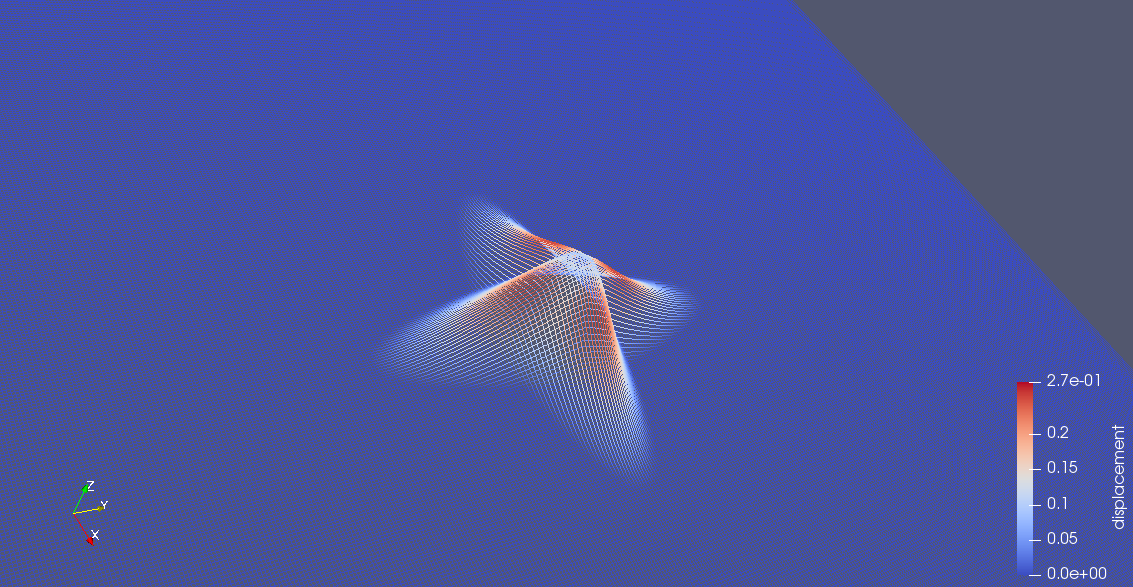
\includegraphics[width=0.8\textwidth]{img/fiber/example_overview.png}
    \caption{Общий вид}
    \label{pic:fiber-example-overview}
\end{figure}

\begin{figure}[H]
    \centering
    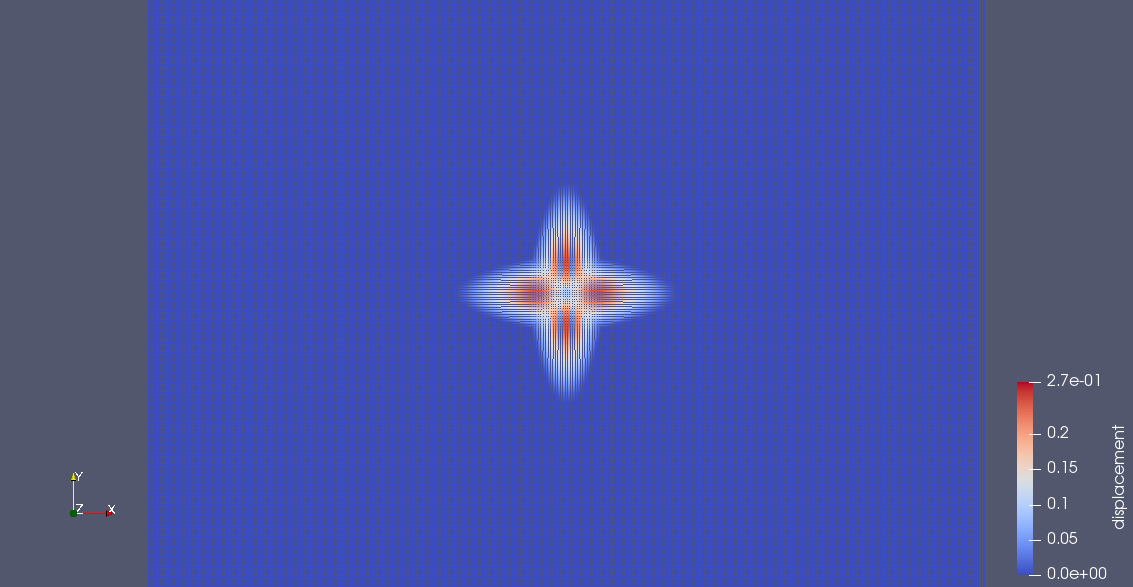
\includegraphics[width=0.8\textwidth]{img/fiber/example_top.png}
    \caption{Вид сверху}
    \label{pic:fiber-example-top}
\end{figure}

\begin{figure}[H]
    \centering
    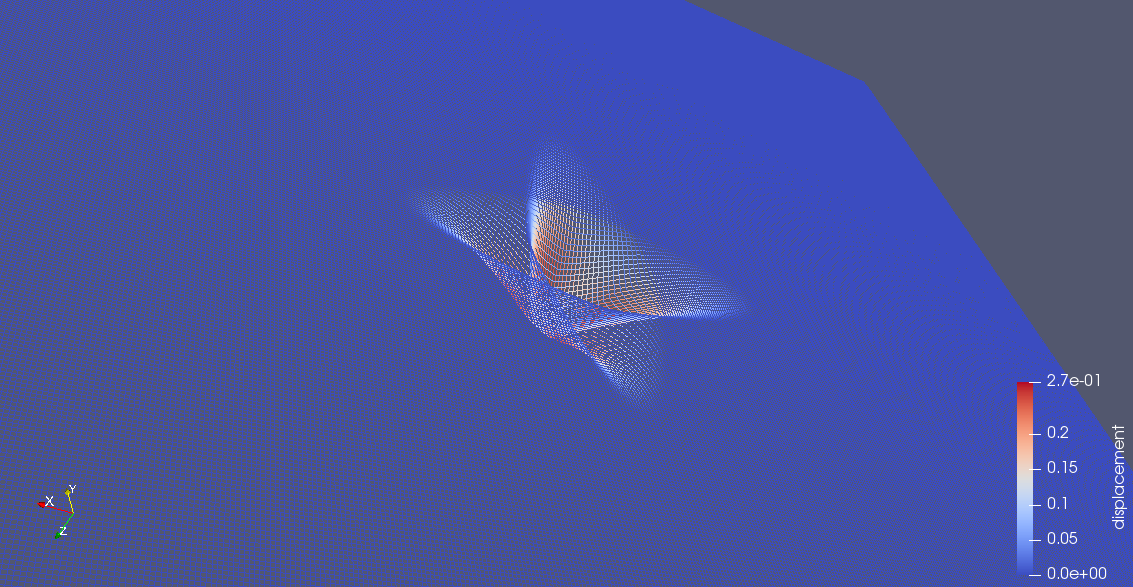
\includegraphics[width=0.8\textwidth]{img/fiber/example_bottom.png}
    \caption{Вид снизу. Виден прогиб ткани в центре.}
    \label{pic:fiber-example-bottom}
\end{figure}

\begin{figure}[H]
    \centering
    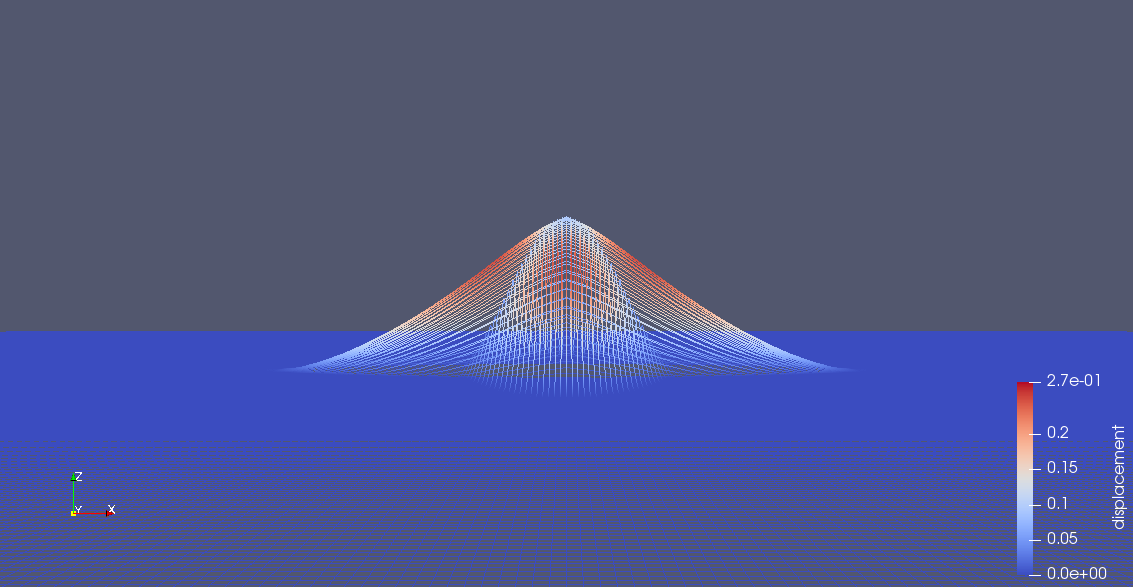
\includegraphics[width=0.8\textwidth]{img/fiber/example_side.png}
    \caption{Вид вдоль нитей}
    \label{pic:fiber-example-side}
\end{figure}

\begin{figure}[H]
    \centering
    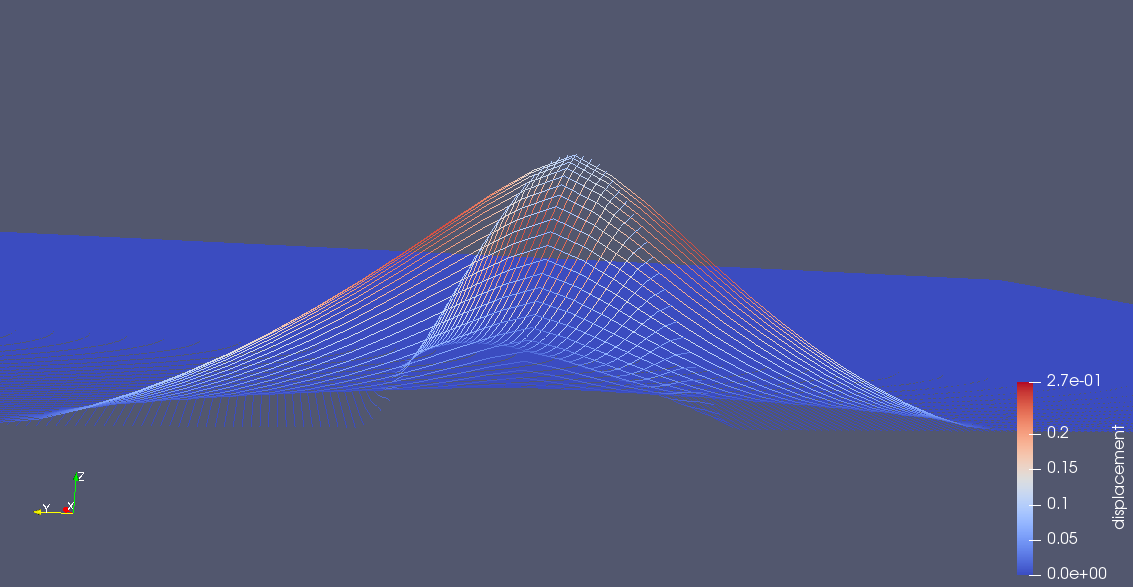
\includegraphics[width=0.8\textwidth]{img/fiber/example_slice.png}
    \caption{Срез вдоль нитей. Видно расслоение утка и основы.}
    \label{pic:fiber-example-slice}
\end{figure}


Большая часть расчётов при различных постановках приводится в~\ref{ch:results}.
